\chapter{Optimization of the cross section for power extraction}

\section{Introduction}

%Galloping occurs as a result of the pressure difference created due to the relative distance between the shear layers and the respective walls of the cross section, at the top and bottom sides of the body. As discussed in section \ref{subsec:c_y and shear layers}, the instantaneous induced angle makes one of the separated shear layers closer to the wall creating a low pressure region. This pressure difference results in a transverse forcing (normal to the direction of the flow) which becomes in phase with the transverse velocity and sustains galloping.  JL: this needs to be re-written. Even I don't really know what you are trying to say here. I think you are mixing up a description of the flow, and the hypothesis that you are going to test.


 Galloping is due to an increase in mean induced lift force \cy\  with an increase in the instantaneous induced angle of attack. This instantaneous angle of attack is directly related to the transverse velocity - an increase in angle of attack implies an increase in velocity. This increase in mean lift force is created by an increase in the difference in mean pressure on the upper and lower sides of the body. The mean pressure on each side of the body is related to the structure of the mean shear layer, in particular to the separation and potential reattachment of this shear layer, and the size of any resulting recirculation region. An increase in angle of attack forces one shear layer (the lower one) closer to the wall, meaning a high speed region is placed close to this wall. A simple consideration of Bernoulli's equation shows that this high speed region should result in a region of low pressure. This low pressure on the upper side results in a positive pressure difference between the lower and upper sides, and thus a positive mean lift The fact that this mean lift occurs as a function of the angle of attack, and therefore the transferse velocity, implies that this transverse forcing should be in phase with the transverse velocity

From equation \ref{eqn:power_alt} discussed in section \ref{subsec:ave_pow} it is clear that the power transferred from fluid to the body is a function of the induced forcing $F_y$ and the transverse velocity $\dot{y}$. The sign of the average power represents the direction of power transfer; positive power represents the power transfer from fluid to the body, negative power represents power transferring from body to the fluid. Thus, according to equation \ref{eqn:power_alt} it can be deduced that if there is a scenario where both high induced forcing and high transverse velocities are present, higher power output can be achieved.

This can be related directly to the shape of the $C_y$ vs. $\theta$ curve. To optimize power
transfer this curve should,

\begin{itemize}
\item have a high gradient $\partial C_y/\partial \theta$ at
  $\theta = 0$
\item a large maximum $C_y$
\item this maximum $C_y$ should occur at a high value of $\theta$
\end{itemize}

All of these features can be influenced by the cross section of the
body which is galloping. Therefore, if the geometric features of the
cross section that influence these curve features can be identified,
an informed search for an optimal cross section for power extraction
can be undertaken. The major features of the body that influence these
$C_y$ vs. $\theta$ curve parameters are discussed below.

\citet{Luo1994}, showed that the afterbody of the cross section has a direct impact on $C_y$ vs. $\theta$ curve. One interesting observation of this study was that inhibiting the shear layer re-attachment results in higher peak induced force coefficient $C_y$ occurring at high induced angles (high transverse velocities). The opposite of this result was discussed by \citet{Robertson2003} where long rectangular cross sections did not exhibit galloping due to shear layer reattachment at low $\theta$. Furthermore, \citet{Luo1994} have discussed the impact of the reattachment of the shear layer at the trailing edge. As $\theta$ is further increased beyond the angle of reattachment, the enclosed ``bubble'' region of the separated reattached shear layer shrinks in size reducing the difference in suction in the top and bottom sides of the body and results in a reduction in \cy (refer section \ref{subsec:c_y and shear layers}). 

Therefore, it could be hypothesised that a higher power transfer could be obtained by inhibiting the shear layer re-attachment. 

Here, the influence of shear layer and its reattachment on the mean power is discussed. It is crucial to keep the shear layer closer to the body for galloping. Thus, a cross section which has a straight initial section (which has initial streamlining) followed by a slanting section to inhibit the shear, layer had to be considered for analysis. Therefore, a cross section which is a hybrid of a square and a triangle was considered. The cross section was transformed gradually by manipulating the ratio of two length scales. This cross section provided the flexibility of gradually inhibiting the shear layer reattachment while having the initial streamlining of the shear layers to sustain galloping. 

The force data are presented for each stationary cross section. This is followed by presentation of extracted power curves, calculate from the QSS model using this force data for each new body. Based on the QSS power data, an optimum cross section for power extraction, from the family of cross sections that have been tested, is identified.

The main features of the generated $C_y$ vs. $\theta$ curves for the
new bodies are identified and linked to the flow structure present by
analysing the mean surface pressure and flow velocity data. Following
this, a comparison is made between QSS and DNS mean power on the cross
section which provides an optimum mean power.

A final summary is presented outlining that the behaviour of the shear layers is a controlling factor for mean power output. The preliminary design considerations to obtain an optimum power output should therefore focus on the manipulation of these shear layers. 





\section{Influence of the shear layers}

In a typical cross section which sustains galloping, the induced lift \cy\ increases with increasing induced angle $\theta$ until it reaches a maximum value of \cy where the shear layer re attachment occurs. The lift force then decreases as $\theta$ is further increased. The underlying mechanism for this behaviour is discussed in detail in section \ref{subsec:c_y and shear layers}.   

\subsection*{Selection of the cross section}

\begin{figure}
\setlength{\unitlength}{\textwidth}

  \begin{picture}(1,0.23)(0,0.74)
    
  \put(0.2,0.76){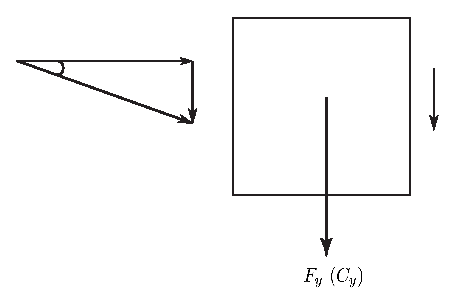
\includegraphics[width=0.5\unitlength]{../FnP/gnuplot/setup-1.eps}}         
      
      
   
 	\put(0.315,0.93){$U$}
 	\put(0.3,0.84){$U_i$}
    \put(0.42,0.88){$\dot{y}$}
    \put(0.28,0.895){ $\theta$}
    \put(0.7,0.87){\small $(+)$}
      	

 	
 	 

     

  \end{picture}

 \caption{Induced angle of attack on the square prism due to the resultant of free-stream velocity of the fluid and transverse velocity of the body.}
    \label{fig:setup_1}
\end{figure}

Several key factors had to be considered during the selection of a suitable cross section for this analysis. These key factors are,

\begin{itemize}
\item The cross section should have a bluff front face with sharp upstream corners for the flow to separate at the leading edges.

\item As the proximity of shear layers to the body plays a vital role in creating \cy\ \citet{Parkinson1989}, the cross section should have a basic level of streamlining.

\item The cross section should consist of a geometric profile in the afterbody, to inhibit or delay the shear layer reattachment.   
\end{itemize}

The square cross section which is considered as the base cross section in this study satisfies the first two criteria of the selection process. Therefore, in order to inhibit the shear layer reattachment the top and bottom sides of the trailing edges of the square was tapered off and a hybrid cross section of a square and a triangle (illustrated in figure \ref{fig:hybrid_section}), i.e, a pentagon was produced. This cross section satisfied all criteria in the cross section selection process. Another advantage of this cross section was the inhibition of the shear layer could be varied systematically by varying one variable which is $\ratio$. The $\ratio$ was changed gradually from 1 to zero at increments of 0.25 where 1 being the square cross section and 0 being an isosceles triangle. 


\section{Static body results}
\label{sec:cross-sec-Static body results}

\begin{table}[ht]

\begin{center}
\setlength{\unitlength}{\textwidth}

\begin{tabular}{c c c c c} % centered columns (4 columns)
\hline\hline %inserts double horizontal lines
\\[0.2ex]
Case & $a_1$ & $a_3$ & $a_5$ & $a_7$ \\ [0.8ex] % inserts table 
%heading
\hline 
\\[0.8ex]% inserts single horizontal line
Re=200 & 2.32 & 197.8 & 4301.7 & 30311.9 \\[0.8ex]% inserting body of the table
Re=22300 & 2.69 & 168 & 1670 & 59900 \\ [1ex] % [1ex] adds vertical space
\hline %inserts single line
\end{tabular}

\caption{Coefficient values used in the 7th order interpolation polynomial for high ($Re=22300$) and low ($Re=200$) Reynolds numbers. These data are used as input data to calculate the right-hand side of Eq. \ref{final_equation_motion} throughout this study.}
 
\label{table:cy-coefficients} % is used to refer this table in the text
\end{center}
\end{table}



Stationary time averaged $C_y$ results were obtained for cross sections where $\ratio=1,0.75,0.5,0.25$ and $0$ using DNS at $\reynoldsnumber=200$. Table \ref{table:cy-coefficients-hybrid} shows the coefficients of the $7^{th}$ order curve fitting for each cross section. In order to achieve a better fit, piecewise interpolation using multiple $7th$ order polynomials were incorporated for a single cross section. During the curve fitting process more importance was given to accurately fitting the positive portion of the $C_{y}$ curve, as the power transfer from the fluid to the body only occurs in this region. 

\begin{figure}
  \setlength{\unitlength}{\textwidth}

  \begin{picture}(1,0.75)(0,0)
    % % %90
      % % % Parkinson Data 
      \put(0.035,0.5){\includegraphics[width=0.5\unitlength]{./FnP/lift_curve_sq.eps}}
      \put(0.495,0.5){\includegraphics[width=0.5\unitlength]{./FnP/lift_curve_075.eps}}
      \put(0.035,0.27){\includegraphics[width=0.5\unitlength]{./FnP/lift_curve_05.eps}}
      \put(0.495,0.27){\includegraphics[width=0.5\unitlength]{./FnP/lift_curve_025.eps}}
      \put(0.3,0.0){\includegraphics[width=0.5\unitlength]{./FnP/lift_curve_tri.eps}}
      
      
   
      
      
%      \put(0.23,0.00){ $\displaystyle\frac{c}{\rho\mathcal{A}U}$}
%      \put(0.73,0.00){ $\displaystyle\frac{c}{\rho\mathcal{A}U}$}

      \put(0.3,0.26){$\theta$}
      \put(0.76,0.26){$\theta$}
      \put(0.56,-0.01){$\theta$}
      
      \put(0.01,0.405){$\displaystyle C_y$}
       \put(0.01,0.65){$\displaystyle C_y$}
      \put(0.3,0.14){$\displaystyle C_y$}
      
      \put(0.106,0.705){\small(a)}
      \put(0.565,0.705){\small(b)}
      \put(0.106,0.475){\small(c)}
      \put(0.565,0.475){\small(d)}
      \put(0.37,0.207){\small(e)}
      

  \end{picture}

  \caption{Induced lift coefficient $C_y$ at different angles for selected cross sections. Data presented for cross sections, (a) square, (b) $\ratio=0.75$, (c) $\ratio=0.5$, (d) $\ratio=0.25$ and (e) triangle.}
  \label{fig:lift_curves}
\end{figure} 

The $C_y$ vs. $\theta$ curves in figure \ref{fig:lift_curves-hybrid} shows that the peak value of \cy\ shifts to the right as $\ratio$ is increased, hence, the peak \cy\ occurs at high induced angles.  These data agree with \citet{Luo1994} where the peak of the maximum \cy\ value was shifted to higher induced angles when reattachment was delayed. As $\theta$ is proportional to the transverse velocity of the body via $\tan{\theta}=\frac{\dot{y}}{U}$, the peak value of \cy\ occurs at high induced velocities as \ratio\ is decreased. Therefore, bodies with a short straight section, or small \ratio, satisfy one of the three conditions required to optimize the power transfer.

However, a complicating factor is the appearance of a negative region on the $C_y$ vs. $\theta$ curves for cross sections where $\ratio\leq0.25$. Here, initially \cy\ decreases as $\theta$ is increased and only increases after reaching a minimum, nonzero value of $\theta$. The presence of this negative portion is an indication of unfavourable power transfer, i.e. power transferred from body to the fluid as the direction of the force and velocity vectors are out of phase. This implies that when the induced angle of attack is low (when the transverse velocity is low), power transfer is from the body to the fluid, but when the transverse velocity is high, power transfer is from the fluid to the body. This means that the direction of power transfer can be different at different points in the oscillation cycle. This will be further discussed in the upcoming section \ref{sec:negative-region}.

 
 
 \section{QSS Mean power output}
 \label{sec:cross-sec-qss-mean power}
 
 % !TeX spellcheck = en_GB
\begin{figure}[!htb]
  \setlength{\unitlength}{\textwidth}

        \begin{picture}(1,0.4)(-0.02,0)

 
      
      \put(0.08,0.02){\includegraphics[width=0.75\unitlength]{./chapter-cross-sections/fnp/mean_power_hyb.eps}}

      \put(0.46,0.00){\massdamp}
      
      
     
       \put(0.03,0.235){$\displaystyle\frac{P_{m}}{\rho \mathcal{A}U^3 }$}
      

      %\put(0.095,0.218){\small(a)}
      %\put(0.565,0.218){\small(b)}
      
    \end{picture}

  \caption{Dimensionless mean power obtained using QSS model as a function of \massdamp. Data presented for five selected cross sections, square ($\triangle$), $\ratio=0.75$ (+), $\ratio=0.5$ (\ding{117}), $\ratio=0.25$ ($\times$) and triangle (\ding{108}) at $\reynoldsnumber=200$, $\massstiff=100$.}
    \label{fig:power_curves}
\end{figure}

 %vspace{10cm}

 
 Mean power output predictions are obtained for these different cross sections using the QSS model and the stationary induced lift data JL: shown in figure BLAH used as inputs to the QSS model. Figure \ref{fig:power_curves} shows the mean power vs. \massdamp\ for different cross sections namely $\ratio=1,0.75,0.5,0.25$ and $0$. The maximum mean power increases until $\ratio=0.25$. This agrees well with the formulated hypothesis JL: what is this hypothesis?. The shear layer re-attachment is delayed as \ratio\ is decreased and an increase in maximum power output could be observed JL: you can't say anything about the shear layer from looking at this graph. As \ratio\ is further decreased to $\ratio=0$ the peak mean power output is reduced. This result goes against the initial hypothesis. Thus, it was further investigated the cause of this reduction in mean power output. 

JL: re-organize this argument. First add some discussion of the features of the figure. Break the discussion into two parts, for data $\ratio > 0.25$, and for $\ratio \leq 0.25$. For the high \ratio\ cases, the trends are basically the same; power first increases with increasing \massdamp, then peaks, and then decreases. Generally, the amount of power increases with a decrease in \ratio. This is what is expected by looking at the curves in figure 2. For the low \ratio\ cases, the trend is different; power first increases with \massdamp, then peaks, and then drops dramatically. The power extracted also appears to decrease with a decrease in \ratio. So, the fact that there are two regimes - high and low \ratio\ - indicates there is a distinct change in the flow structure. Note that you have already seen evidence of a change in flow structure - the appearance of a negative region on the lift curve for these low \ratio\ cases. This fact is further investigated in section PUT IN REF.
 
It was identified in section \ref{sec:cross-sec-Static body results} the presence of a negative portion of the $C_y$ vs. $\theta$ curve at $\ratio\leq0.25$. It was established in that section that the presence of this negative portion of the $\cy$ vs. $\theta$ curve results in unfavourable power transfer i.e. power transfer from the body to the fluid. Inspection of the lift curves in figure \ref{fig:lift_curves-hybrid} (d) and (e), shows that the negative region of the curve - the range of $\theta$ over which \cy\ is negative - increases as \ratio\ is decreased. An argument could be that when \cy\ becomes negative it will preclude galloping altogether. This argument is partially true. However, manipulating the initial condition (initial transverse velocity) will somewhat rectify this problem. If an initial velocity which would make a positive induced angle is given galloping would sustain. This is how the mean power data were obtained for $\ratio=0.25$ and $\ratio=0$. That being mentioned to sustain galling another crucial factor is damping \citet{Paidoussis2010}. This is the reason why even though a higher initial condition is given the range of \massdamp\ for power production is short for $\ratio=0.25\ \text{and}\ 0$ compared to other tested cross sections. 

JL: KASUN, you need to look through the literature for discussions of ``hard'' and ``soft'' galloping. What you are describing is the fact that the transition to galloping can be hysteretic. It might not start naturally from amplitude of zero, but if you give the body a push (manipulate initial conditions), it will self-sustain galloping. Does this make a difference to the extracted power curves you've presented in figure 3.3? Is there a range of \massdamp\ where you can get either very high power, or close to zero, depending on the initial conditions you start with? You could show both values and give an indication of the size of the hysteresis loop.

\section{Presence of the negative region of the $\cy$ vs. $\theta$ curves}
 \label{sec:negative-region}

As a reduction in power was observed in some cross sections due to the presence of a negative portion of the $\cy$ vs. $\theta$, further investigations were carried out in order to understand the underlying reasoning for this phenomenon.

KASUN: This style of writing is too ``familiar''. First I think this section should be renamed something like ``Investigation of hysteretic response for low \ratio''. Then the intro paragraph can point out that there is a negative region in the lift curves, and an apparent hysteresis in the power curves pointing to a change in flow regime that you are going to investigate further here.

\subsection{Surface pressure}
\label{subsec:cross-sec-surface pressure}

As the driving force of the galloping body is the pressure forces created from the relative distances of the shear layers JL: distance between the shear layers? How about ``pressure on the upper and lower sides which is related to the behaviour of the shear layers''?, the primary investigation was carried out analysing surface pressure data on the time averaged stationary data of the cross section. The test cross section taken here out of the cross sections was the isosceles triangle ($\ratio=0$) as it produced the largest negative region out of the cross sections tested for mean power output. 

KASUN: you need to state what you are doing.
\begin{itemize}
\item Attempting to link the appearance of a negative region in the
  lift curve to a change in flow structure
\item Take the triangle case as representative of the low \ratio\
  cases
\item First thing to investigate is the distribution of pressure along
  the two rear surfaces.
\end{itemize}

Time averaged (to filter out the influence of vortex shedding) surface pressure data  on the top and bottom surfaces of the cross sections at $\theta=4^{\circ}$, $\theta=16^{\circ}$ and $\theta=21^{\circ}$ were obtained for the isosceles triangle. By having a closer look at the \cy\ vs. $\theta$ curves it could be seen that these points correspond to a negative \cy\ that is further decreasing with increasing $\theta$, a negative \cy\ that is increasing with increasing $\theta$ and a significantly positive value of \cy.

KASUN: expand. What is the value of $\theta$ where the lift force becomes positive again? 
 
\begin{figure}
  \setlength{\unitlength}{\textwidth}

        \begin{picture}(1,1.1)(0,0.35)

      % % % Parkinson Data 
      \put(0.1,1.1){\includegraphics[width=0.75\unitlength]{./chapter-cross-sections/fnp/surf-pres-tri-4.eps}}
      \put(0.1,0.737){\includegraphics[width=0.75\unitlength]{./chapter-cross-sections/fnp/surf-pres-tri-16.eps}}
      \put(0.1,0.38){\includegraphics[width=0.75\unitlength]{./chapter-cross-sections/fnp/surf-pres-tri-21.eps}}
     
      
      



%      
    \put(0.21,1.41){\small(a)}
     \put(0.21,1.05){\small(b)}
     \put(0.21,0.69){\small(c)}
\put(0.1,0.95){$\displaystyle P_{s}$}
\put(0.1,1.3){$\displaystyle P_{s}$}
\put(0.1,0.56){$\displaystyle P_{s}$}
\put(0.26,0.35){Relative destance from the leading edge}

      
    \end{picture}

    \caption{Surface pressure of top (\ding{83}) and bottom (\ding{117})  surfaces of the static triangular cross section at (a) $\theta=4^\circ$, (b) $\theta=16^\circ$ \ and (c) $\theta=21^\circ$ A clear pressure difference is visible between the surfaces. The top surface comparatively has more negative pressure where a lift is created which results in a negative $C_y$ at $4^\circ$ and reduces as $\theta$ \ is increased, while the vice versa occurs at the top surface.}
    \label{fig:surf_pres}
\end{figure}

 %vspace{10cm}
 

KASUN: in the figure, why do you plot as a function of X? Wouldn't it be better to plot as a function of the distance along the surface from the front edge (so all the plots would cover the same range)? Wouldn't it be even better to show an image of the triangle and the pressure as a contour relative to the surfaces? See image about halfway down this page: \url{http://www.heliciel.com/en/aerodynamique-hydrodynamique/profils\%20aile\%20profil\%20pale.htm} As it is I don't think these plot mean very much because the direction of force for each surface is different.

KASUN: also, shift the pressure values up so that they are all positive (add 1.2 to everything) it will make everything easier to interpret that dealing with negative pressures, and makes absolutely no difference to your conclusions. Or find the pressure at the inlet of the domain, and subtract that as your reference pressure.
 
Figure \ref{fig:surf_pres} shows the surface pressure of the top and bottom surfaces of the body ($\ratio=0$) starting from  the leading edges. At $\theta=4^{\circ}$, the pressure of the bottom of the body is greater than the top. Therefore, a pressure difference is created and a force is generated in the upward direction which according to the sign convention presented in \ref{fig:induced_lift_sketch}, is against the velocity of the body, hence giving a negative $\cy$. As $\theta$ (figure \ref{fig:surf_pres} (b)) is increased, to $16^{\circ}$ the gap between the surface pressure at the leading edge between the top and the bottom reduces. This effect results in a reduction of the magnitude of $\cy$ (although it is still negative). As $\theta$ is further increased at $21^{\circ}$ (figure \ref{fig:surf_pres} (c)) the surface pressure on the top side becomes greater than the bottom. Therefore, the net effect of the pressure difference is a positive $\cy$ which the driving force $F_y$ in phase with the velocity of the body.

KASUN: are you sure you have the sign convention right here?

KASUN: can you add a summarizing paragraph for this section? Why is this important? What have you shown here? That the direction of the force depends on the direction of the pressure gradient? We knew that already.

\subsection{Velocity profiles at the points of flow separation}

The most important points of a cross section under galloping are the two flow separation points of the leading edges of the cross section, where a significant pressure difference occur JL: a pressure difference between the two separation points? What evidence do you have that these are the ``most important'' points? Considering all of the discussion so far in this chapter has focussed on reattachment, I would think that the reattachment points are the most important points. A key variable which directly relates to the fluid dynamic pressure is the velocity of the fluid. Although not strictly true in all cases of viscous flows, one should expect that a higher flow speed correspond with a lower pressure from basic fluid dynamic theory. By measuring the flow velocity behaviour at, or near, the separation points, the cause of the pressure differences that occur along the upper and lower surfaces shown in section (SEE ABOVE) can be found.

\begin{figure}[!htb]
\setlength{\unitlength}{\textwidth}

  \begin{picture}(1,0.38)(0,0.74)
    
  \put(0.4,0.76){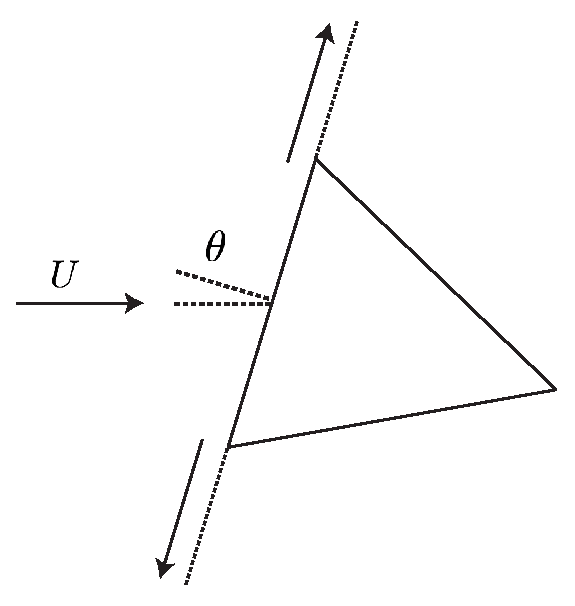
\includegraphics[width=0.25\unitlength]{./chapter-cross-sections/fnp/tri-sketch.eps}}         
      
      
   
 	\put(0.38,0.937){$\theta$}
 	%\put(0.52,0.74){$l$}
   

 	
 	 

     

  \end{picture}

 \caption{Illustration of the lines along which the flow velocity magnitudes have been extracted. The data have been extracted along a line starting from the separation points in the outward direction (shown with arrows) for the top and bottom surfaces.}
    \label{fig:tri-sketch}
\end{figure}
   
Mean velocity magnitude data of the flow were obtained along two lines parallel to the front wall of the cross section one stating at the top and the other stating at the bottom leading edges of the cross section spreading outward as illustrated in figure \ref{fig:tri-sketch}. The lengths of these lines were equal to the width of the cross section. Data were obtained for the same cases presented earlier i.e. isosceles triangle ($\ratio=0$) at $\theta=4^{\circ}$, $\theta=16^{\circ}$ and $\theta=21^{\circ}$.
       
\begin{figure}
  \setlength{\unitlength}{\textwidth}

        \begin{picture}(1,1.1)(0,0.35)

      % % % Parkinson Data 
      \put(0.1,1.1){\includegraphics[width=0.75\unitlength]{./chapter-cross-sections/fnp/vel_prof-tri-4.eps}}
      \put(0.1,0.737){\includegraphics[width=0.75\unitlength]{./chapter-cross-sections/fnp/vel_prof-tri-16.eps}}
      \put(0.1,0.38){\includegraphics[width=0.75\unitlength]{./chapter-cross-sections/fnp/vel_prof-tri-21.eps}}
     
      
      



%      
    \put(0.21,1.41){\small(a)}
     \put(0.21,1.05){\small(b)}
     \put(0.21,0.69){\small(c)}
\put(0.1,0.95){$\displaystyle V_m$}
\put(0.1,1.3){$\displaystyle V_m$}
\put(0.1,0.56){$\displaystyle V_m$}
\put(0.34,0.35){Distance from the leading edge}

      
    \end{picture}

    \caption{Velocity magnitudes of the flow along a line parallel to the front surface spreading towards top (\solidrule) and bottom (\dashedrule) boundaries (figure \ref{fig:tri-sketch}). These two lines (for the top and bottom surfaces) start from the top and bottom leading edges of the triangular cross section. Data present (a) $\alpha=4^\circ$, (b) $\alpha=16^\circ$ \ and (c) $\alpha=21^\circ$.}
    \label{fig:surf_pres}
\end{figure}

 %vspace{10cm}


KASUN: Does the velocity go back to zero at 0 distance? Why not show
the whole range of $V_m$?

Also, pick a symbol for the distance rather than writing ``Distance
from the trailing edge'', and show this symbol on the graph and the
sketch.

Also, you realise you have used $\alpha$ in the caption of angle of
attack, but the rest of your thesis uses $\theta$?

The velocity profiles at the chosen three incident angles are presented in figure \ref{fig:vel-profile}. A sudden rise of velocity magnitude could be observed at the flow separation points JL: at the separation points the velocity is, and must be, zero. I think what your profiles show is the formation of a wall jet. The maximum velocity magnitude in the top wall jet at $\theta= 4^{0}$ (figure \ref{fig:vel-profile} (a)) is higher than that in the corresponding bottom wall jet, leading to a lower pressure at the top edge. However, the velocity magnitude in the bottom wall jet becomes greater than that in the top wall jet at $\theta=16^{\circ}$. The difference between the top and bottom velocity magnitude in these wall jets tends to increase as $\theta$ is increased to $21^{\circ}$, where the velocity magnitude at the bottom is greater than at the top (figure \ref{fig:vel-profile} (c)). This effectively creates the pressure difference created in figure \ref{fig:surf_pres} (c), which leads to a positive \cy\ and results in a forcing which is in phase with the velocity of the body. 

KASUN: I am not convinced by this. I can see that the magnitude of the upper jet increases with $\theta$, but the lower one seems almost unaffected. I can also see that the maximum of the upper jet first moves towards the surface, then away again. How does this fit with your basic Bernoulli argument?

Why do you need profiles at all? Why can't you plot contours of velocity magnitude? In fact, you could also replace figure 3.4 with plots of pressure contours. Or keep what you have but add plots of contours. I think this whole section would also be stronger if you contrasted a low \ratio\ case (the triangle) with a high \ratio\ case (the square).

Also, why does the dotted line change format between a and b?


\subsection{Mean streamlines}

\begin{figure}[!h]

  \setlength{\unitlength}{\textwidth}

  \begin{picture}(1,0.35)(0,0.725)

    \put(-0.01,0.76){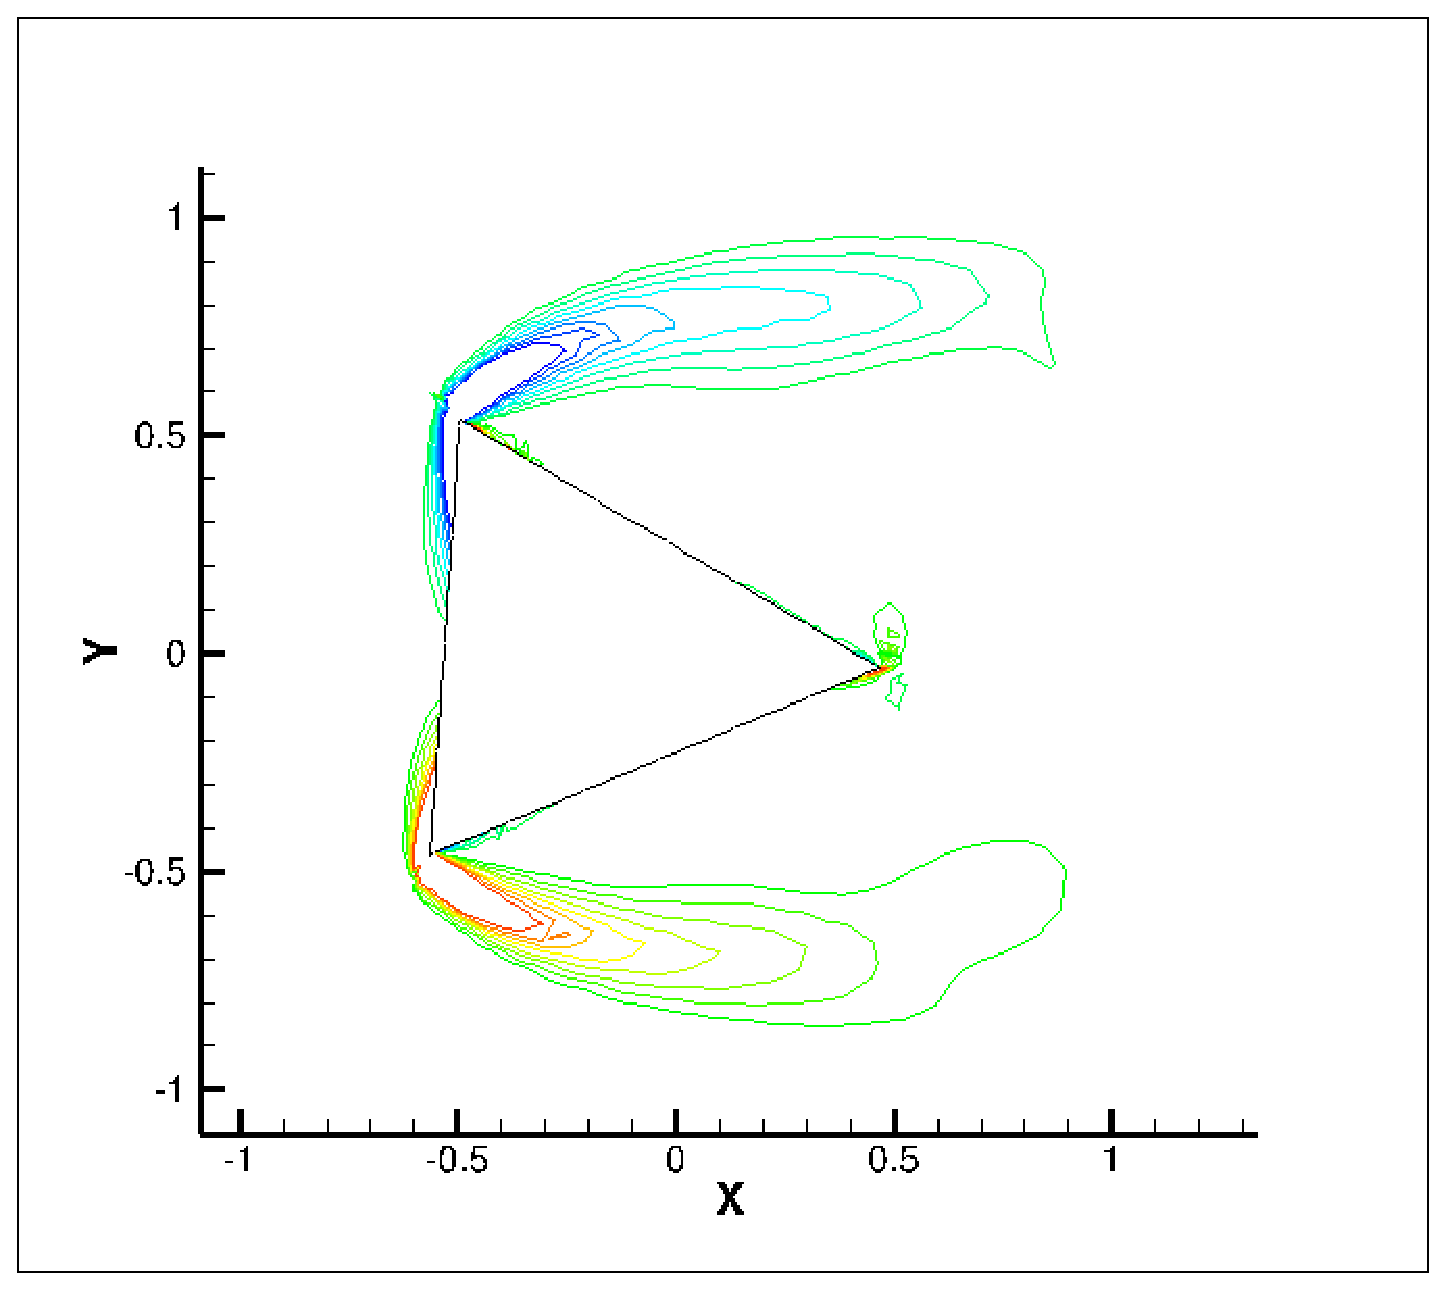
\includegraphics[width=0.33\unitlength]{./chapter-cross-sections/fnp/4.eps}}
    \put(0.335,0.76){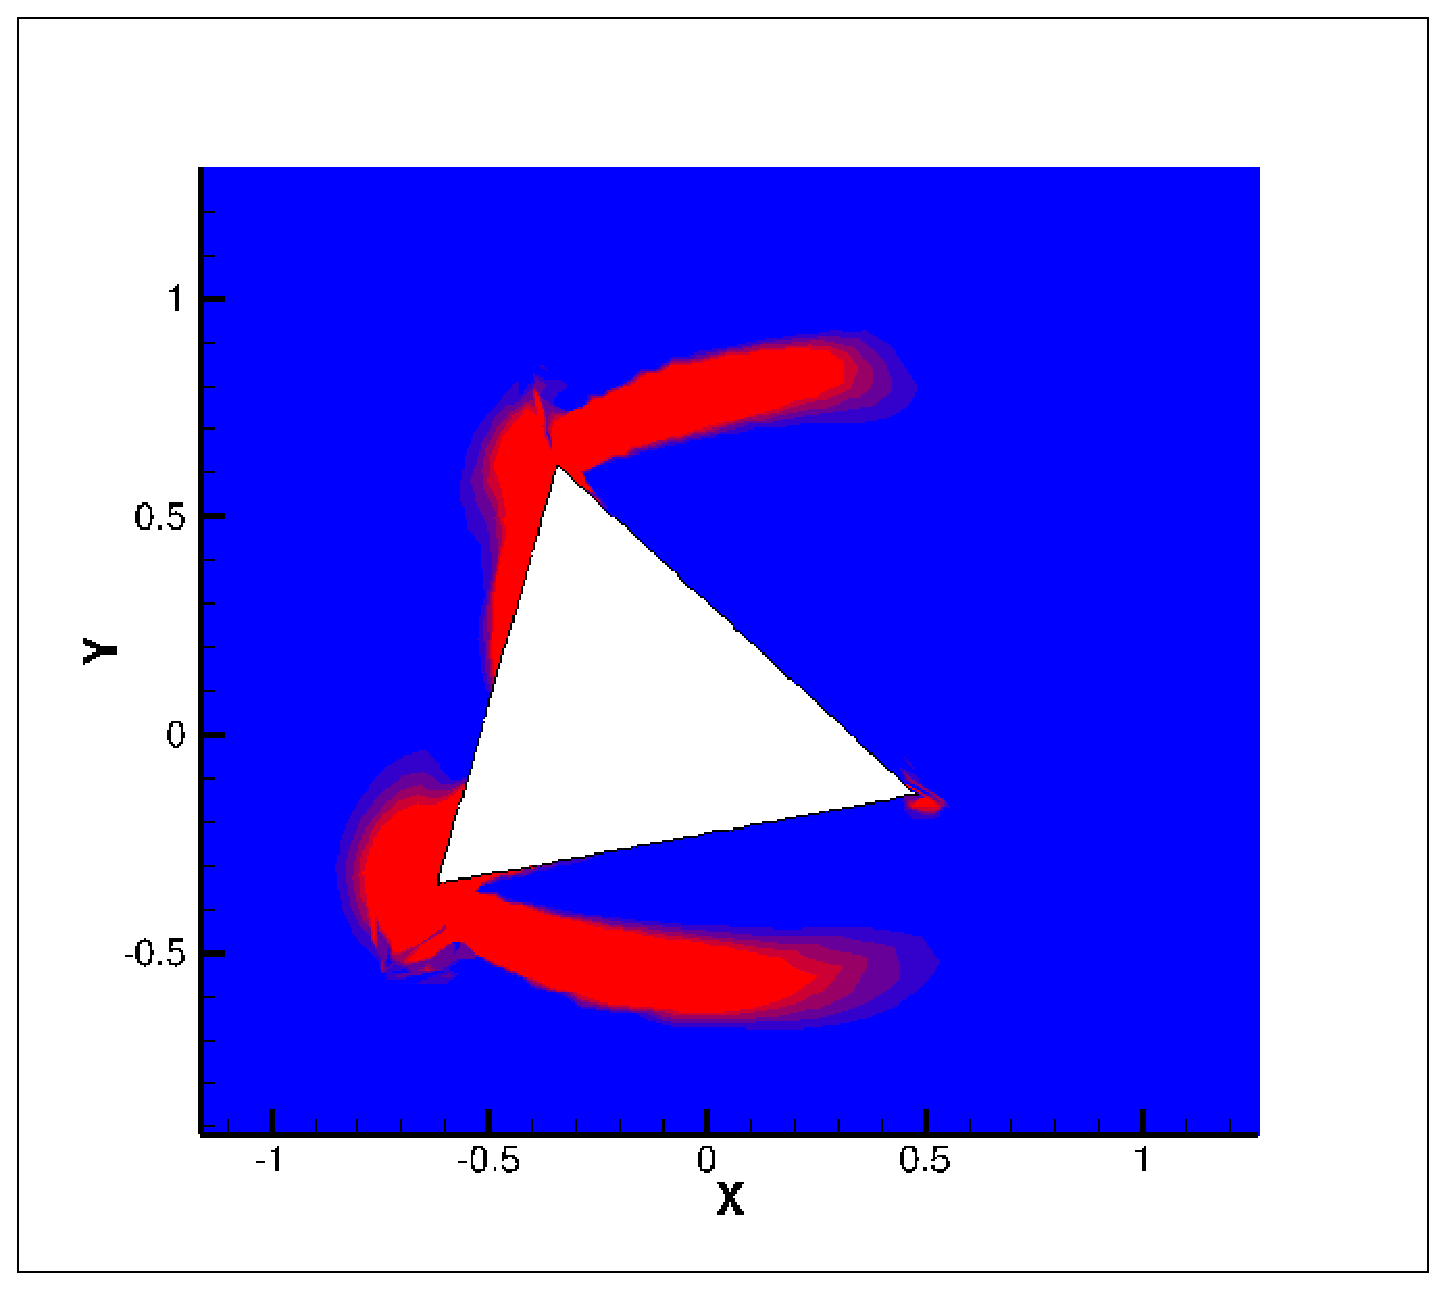
\includegraphics[width=0.33\unitlength]{./chapter-cross-sections/fnp/16.eps}}
    \put(0.68,0.76){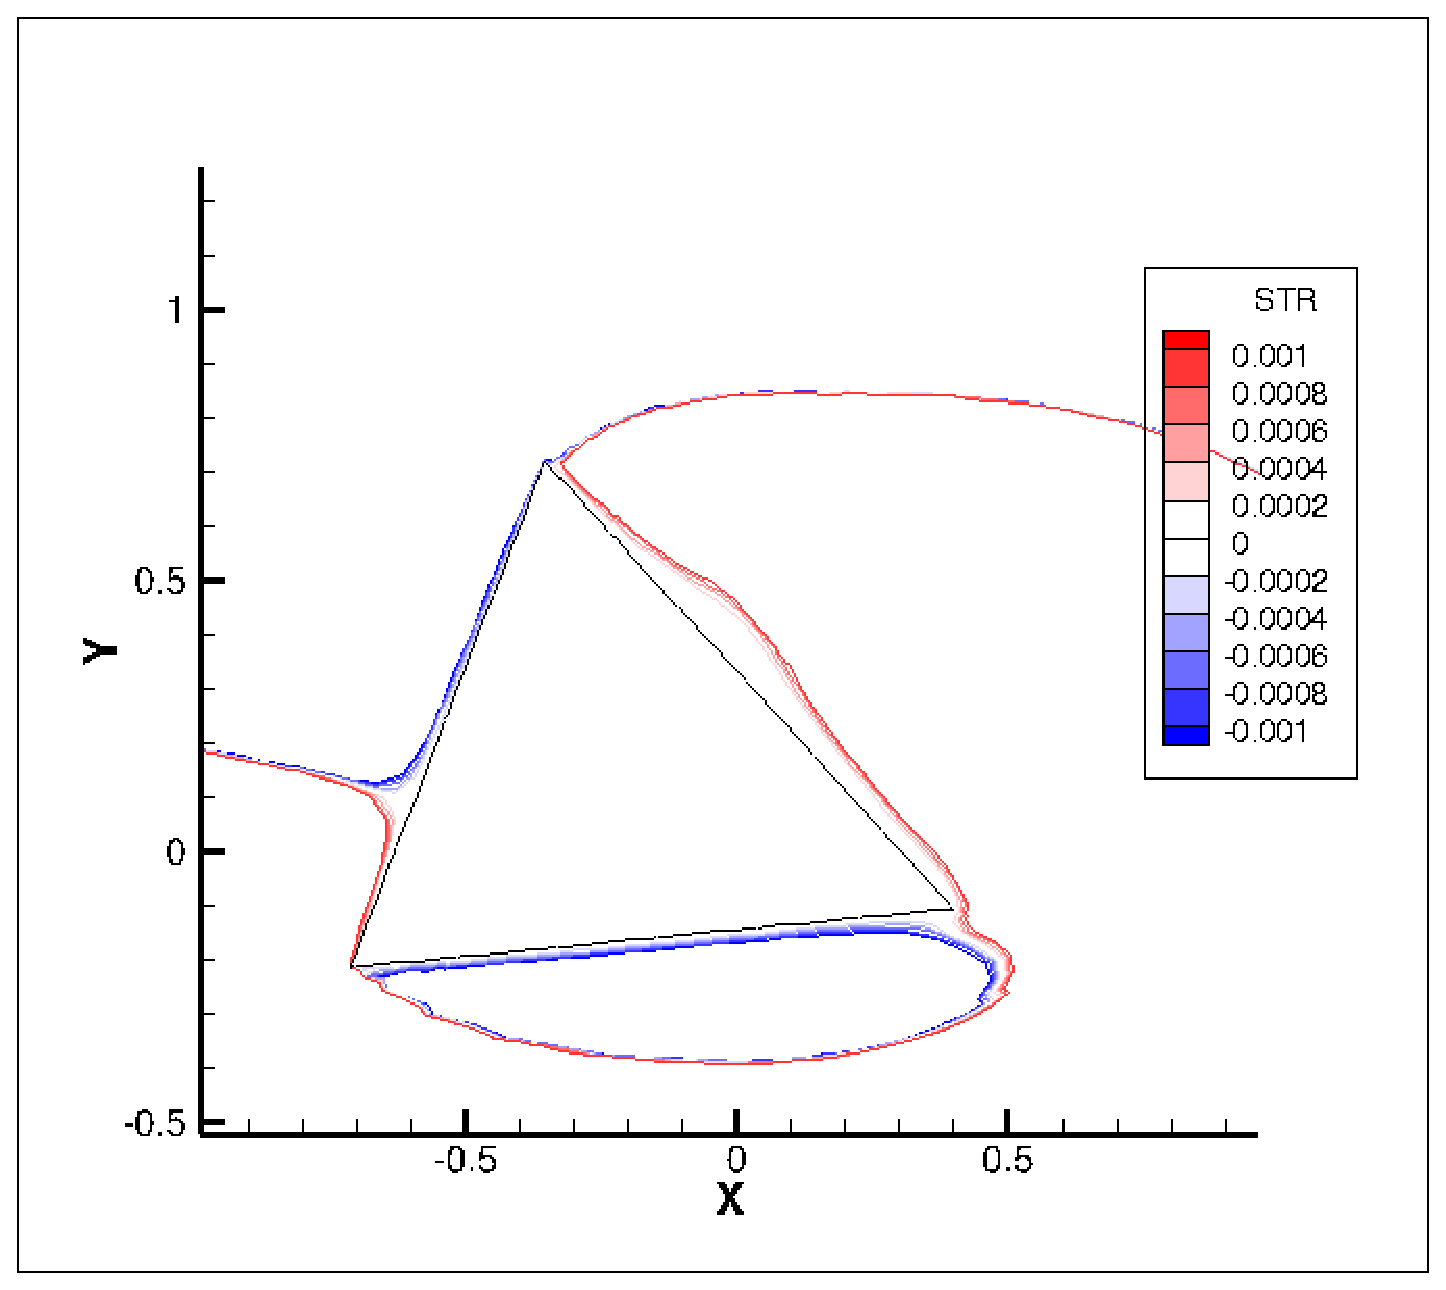
\includegraphics[width=0.33\unitlength]{./chapter-cross-sections/fnp/21.eps}}

   
    
    \put(0.0,0.735){(a)}    
    \put(0.34,0.735){(b)}
    \put(0.685,0.735){(c)}
  
  \end{picture}

  \caption{Contours of the magnitude of the shear strain rate of time averaged flow field on the  stationary isosceles triangle ($\ratio=0$) at $\reynoldsnumber=200$ at different incidence angles. (a) $4^{\circ}$ ( negative value of \cy\ that is further decreasing with increasing $\theta$), (b) $16^{\circ}$ ( negative value of \cy\ that is increasing with increasing $\theta$) and (c) $21^{\circ}$ (a significantly positive value of \cy). The bottom shear layer comes closer to the bottom wall and as the angle of incidence increases.}
  \label{fig:triangle-shear_layers}
\end{figure}




  


Why are the streamlines coloured? Does this add anything?

Do you need the axes and the axis labels?

Do you need the legend?

Keep the field of view the same for each image. As it is the triangle
is a different size in each image. Use this same field of fiew for any pressure and velocity contour plots you make for the sections above.

Keep the streamlines you draw in the field of view. Currently b ``crops'' tne streamlines

The stream functions of the time averaged flow-field of the stationary isosceles triangle at  $\theta=4^{\circ}$, $\theta=16^{\circ}$ and $\theta=21^{\circ}$ are presented in figure \ref{fig:triangle-shear_layers}. Here, it can be observed that the proximity of the bottom shear layer increases as $\theta$ is increased from $4^{\circ}-21^{\circ}$. JL: proximity to what? How do I identify the ``shear layer'' from the streamlines? Would magnitude of the strain rate tensor be better as it shows shear strain rate (and therefore shear stress) directly

\begin{equation}
\epsilon = \frac{1}{2}
\begin{bmatrix}
  2\frac{\partial u}{\partial x} & \frac{\partial u}{\partial y} + \frac{\partial v}{\partial x} \\
  \frac{\partial v}{\partial x} + \frac{\partial u}{\partial y} & 2\frac{\partial v}{\partial y} \\
\end{bmatrix}
\end{equation}

so

\begin{equation}
  |\epsilon| = \frac{1}{2}\left(4\frac{\partial u}{\partial x}\frac{\partial v}{\partial y} + \left(\frac{\partial u}{\partial y} + \frac{\partial v}{\partial x}\right)^2\right)
\end{equation}

By comparing the pressure and the velocity plots together with the stream function flow-field data, it could be seen \cy\ is governed by two mechanisms. Initially at $\theta= 4^{\circ}$ an uneven distribution of the flow is created due to the profile and the positioning (angle of attack) of the geometry creating a forcing ($F_{y}$) similar to the generation of lift of an aerofoil. Comparing figure \ref{fig:triangle-shear_layers} (a) to (b) and (c) the proximity of the bottom shear layer low and hence, does not create a significant pressure force form the relative proximities of the top and bottom shear layers. Therefore, the aerofoil effect becomes more dominant.  

As $\theta$ is increased from $\theta=16^{\circ}$ to $21^{\circ}$, the proximity of the bottom shear layer to the wall of the body increases (figure \ref{fig:triangle-shear_layers} (b) and (c)), and thus becoming the more dominant forcing of the system. This uneven flow distribution as discussed earlier and in \ref{subsec:c_y and shear layers}in detail, creates the positive region of the \cy\ vs. $\theta$ curve.

KASUN: I don't really follow any of this argument. Can you spell it all out in dot points before we go back to writing it? I'm sure there is a logical argument, but you haven't put that argument here.
 
 
 
 
 



